% !TEX root = thesis.tex

\section{Results}\label{sec:results}
\subsection{Driving behavior}
Figures~? (from \citet{DeMooij2021}) and~? (from \citet{Kelapanda2021}) show behavioral results.
[Explanation of what we see in their plots.]

\subsection{Pupil size}
\begin{figure}
  \centering
  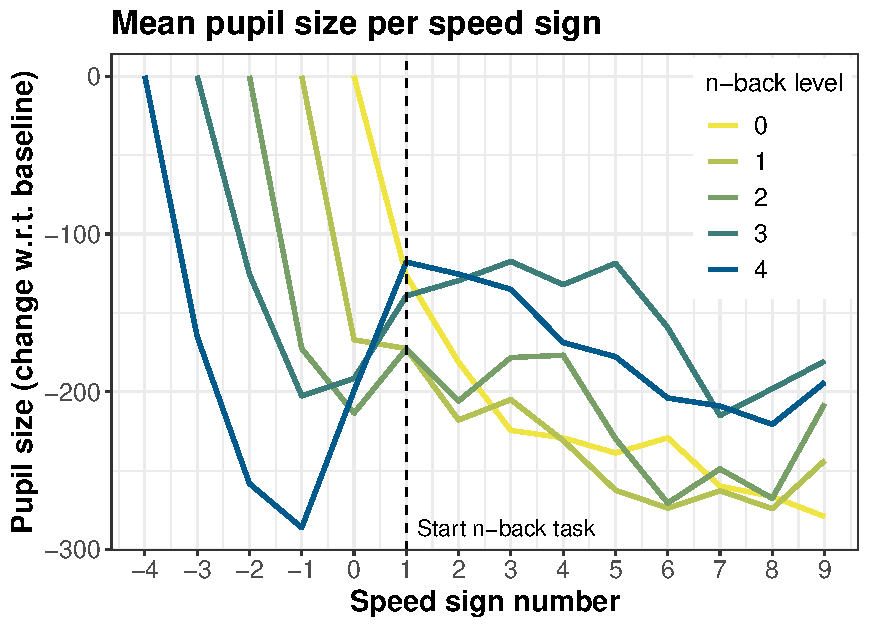
\includegraphics[width=7.5cm]{images/speed_sign_nback.pdf}
  \caption{Mean pupil size over the period between the appearance of two speed signs (\textit{n}\ =\ 25).
  The dashed vertical line indicates the moment that participants need to start regulating their speed according to the speed signs.
  Pupil size was corrected using subtractive baseline correction and is shown in arbitrary units. 
  The data were smoothed using the loess method.}
  \label{fig:ps-speed-sign}
\end{figure}

Figure~\ref{fig:ps-speed-sign} shows how the pupil size of participants changed within a trial.
There is a visible distinction between change in pupil size for low \nback levels (\(n = 0,1,2\)) and high \nback levels (\(n = 3,4\)):
whereas high \nback levels show a peak in pupil size, low \nback levels show a decline from the start of the task.
This difference, which can be characterized as an interaction between \nback level and speed sign number on pupil size, is significant according to an ANOVA with repeated measures [\(F(4,2536)=7.42,\ p < .001\)].

\begin{figure}
  \centering
  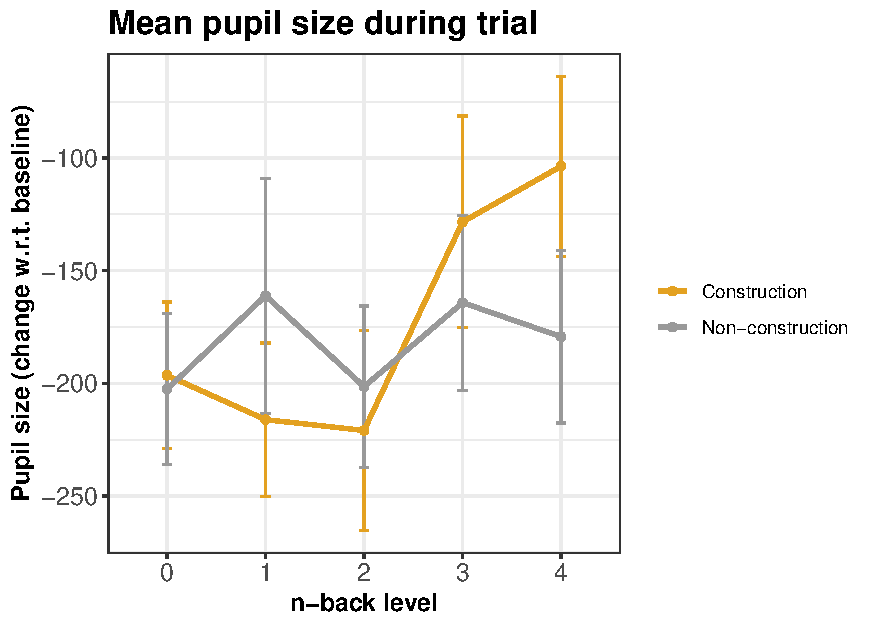
\includegraphics[width=7.5cm]{images/pupil_size_interaction.pdf}
  \caption{Mean pupil size during trial (\textit{n}\ =\ 25); bars represent standard error.
  Pupil size was corrected using subtractive baseline correction and is shown in arbitrary units.}
  \label{fig:mean-ps}
\end{figure}

Figure~\ref{fig:mean-ps} shows the mean pupil size over an entire trial. 
It suggests that there is no effect of \nback on pupil size within the non-construction trials.
For the construction trials there seems to be an increase of pupil size by \nback level more so than for non-construction trials.
However, this suggested interaction between \nback level and construction on pupil size is not significant [\(F(4,216)=1.50,\ p=.20\)].
Disregarding the difference between construction and non-construction we do find a marginally significant effect of \nback level on pupil size [\(F(4,221)=2.39,\ p=.052\)].

\subsection{Fixations on speedometer}

\begin{figure}
  \centering
  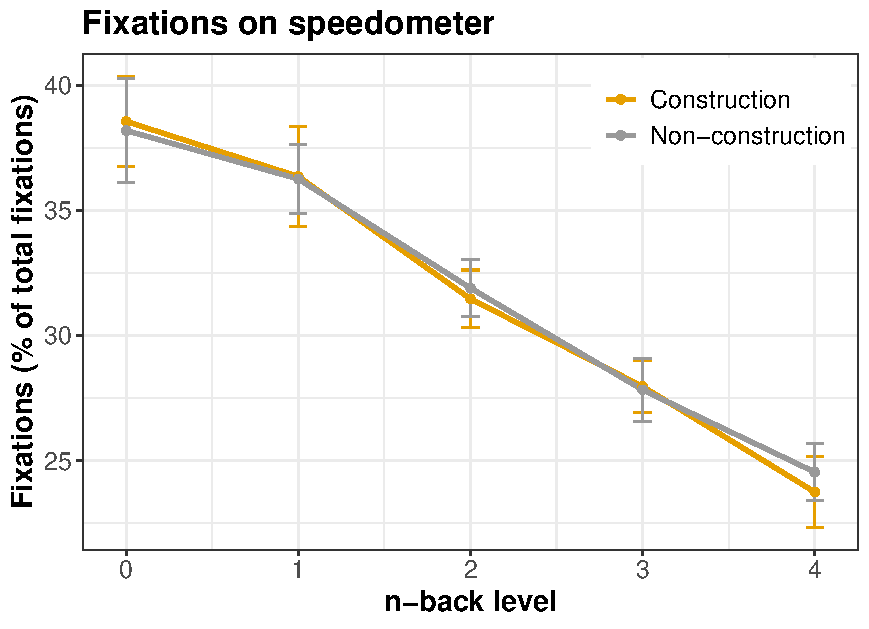
\includegraphics[width=7.5cm]{images/speedometer_interaction.pdf}
  \caption{Number of fixations on the speedometer as a percentage of the total number of fixations for that trial (\textit{n}\ =\ 25); bars represent standard error.}
  \label{fig:fix-speedometer}
\end{figure}

Figure~\ref{fig:fix-speedometer} shows the number of fixations on the speedometer as a percentage of the total number of fixations for a trial.
Like this figure suggests, there is a significant negative correlation between \nback level and fixations on the speedometer [\(F(4,221)=84.72,\ p<.001\)] and no effect of construction or an interaction between \nback and construction. 